% ---------------------------------------------------------------- %

\begin{exercise}[Simulation of test-power]

Simulate the test-power in the two-sample $t$-test: \\
Let $X_1, \dots, X_n, Y_1, \dots, Y_n$ be independent random variables with $X_i \sim N(0, \sigma^2)$ and $Y_i \sim N(d, \sigma^2)$ for all $i = 1, 2, \dots, n$.
Let the null hypothesis be $H_0: d = 0$ and the significance level $\alpha = 5 \%$.
Simulate the test-power (by computing the relative frequency of rejections) for $d \in \Bbraces{-5, -4.5, -4, \dots, 5}$ in $1000$ sumulations each.
Use the parameters

\begin{enumerate}[label = (\alph*)]
    \item $n = 10$ and $\sigma = 3$
    \item $n = 20$ and $\sigma = 3$
    \item $n = 20$ and $\sigma = 1$
\end{enumerate}

for each of which you plot the testpower again $d$.
Comment on your graphic.
Hint:
You can access the $p$-value with \texttt{t.test()\$p.value.}

\end{exercise}

% ---------------------------------------------------------------- %

\begin{solution}

The test reads

\begin{align*}
    H_0: d = 0
    \quad
    \textit{vs}
    \quad
    H_1: d \neq 0,
\end{align*}

Note that

\begin{align*}
    Z := X - Y \sim N(-d, \sigma^2).
\end{align*}

Our test statistic is

\begin{align*}
    T
    =
    \frac{\bar Z + d}{S / \sqrt n}
    \approx
    \frac{\bar Z + d}{\sigma / \sqrt n}
    =
    \frac{\bar Z - (-d)}{\sigma / \sqrt n}
    \sim
    t(n-1).
\end{align*}

We accept $H_1$ iff, for the realization $t$ of $T$,

\begin{align*}
    \alpha
    & >
    \text{$p$-value}
    =
    P_0(|T| \geq |t|)
    =
    2 P_0(T \geq |t|)
    =
    2 (1 - F_T(|t|)) \\
    \iff
    1 - \alpha / 2 & < F_T(|t|) \\
    \iff
    t_{\alpha/2, n-1} & < |t| = \frac{\bar z + 0}{s / \sqrt n}.
\end{align*}

Finally, recall that the power of our test is the probability of accepting $H_1$ if $H_1$ is true.
We will approximate the probability by approximating the expected value by virtue of the LLN.

\begin{figure}[H]
    \centering
    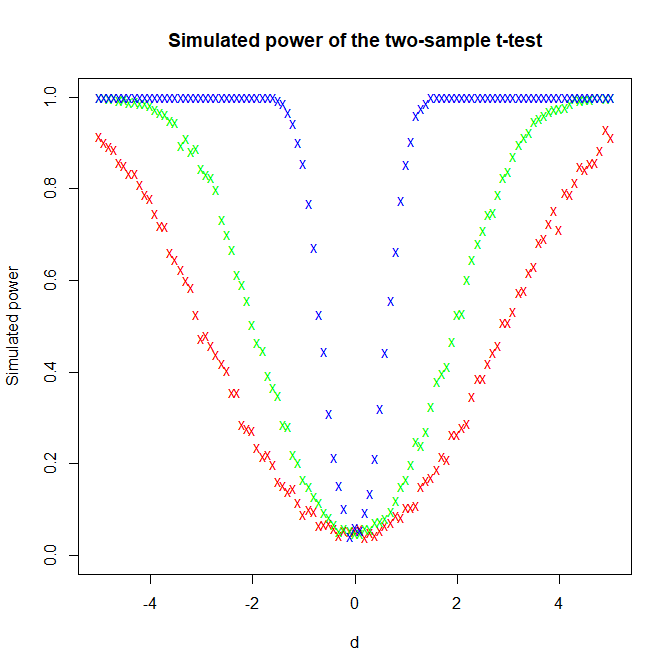
\includegraphics[width = 0.75 \textwidth]{11.3.png}
    \caption{(a) is red, (b) is green and (c) is blue}
    \label{fig:jojojo}
\end{figure}

\lstinputlisting{11.3.r}

\end{solution}

% ---------------------------------------------------------------- %